\documentclass{standalone}
\usepackage{tikz}
\usetikzlibrary{matrix,positioning,fit}
%\usetikzlibrary{shapes.misc}
\usetikzlibrary{decorations.pathreplacing}  % bracket

\definecolor{blue_out}{RGB}{108, 142, 191}
\definecolor{blue_fil}{RGB}{218, 232, 252}
\definecolor{red_out}{RGB}{184, 84, 80}
\definecolor{red_fil}{RGB}{248, 206, 204}
\definecolor{green}{RGB}{130, 179, 102}
\definecolor{yellow}{RGB}{215, 155, 0}
\definecolor{purple}{RGB}{150, 115, 166}
\definecolor{yellow_rec}{RGB}{255, 248, 229}
\definecolor{green_rec}{RGB}{233, 243, 233}

\newcommand\hgt{50pt}
\newcommand\wid{70pt}
\newcommand\rad{15pt}
\tikzset{blue_neuron/.style = {circle, inner sep=0pt, minimum size=2*\rad, draw=blue_out, fill=blue_fil, line width=1.5pt}}
\tikzset{red_neuron/.style = {circle, inner sep=0pt, minimum size=2*\rad, draw=red_out, fill=red_fil, line width=1.5pt}}
\tikzset{mypath/.style = {line width=1pt, -stealth}}
\begin{document}

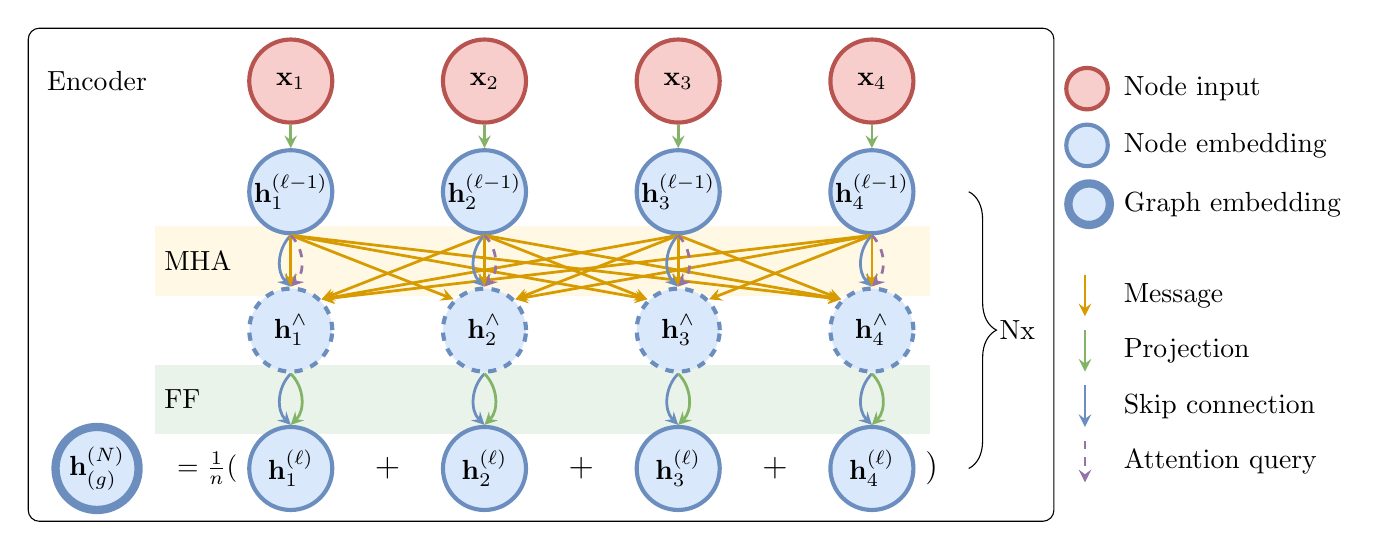
\begin{tikzpicture}
\node[fill=green_rec,inner sep=0,label={[anchor=west]west:FF},  fit={(0.3*\wid,\rad-0.05*\hgt)(4.3*\wid,1.05*\hgt-\rad)}] {};
\node[fill=yellow_rec, inner sep=0, label={[anchor=west]west:MHA},  fit={(0.3*\wid,\rad+0.95*\hgt)(4.3*\wid,2.05*\hgt-\rad)}] {};
\node (Encoder) at (0,2.8*\hgt) {Encoder};
\draw [decorate,decoration={brace,amplitude=10pt,mirror}] (4.5*\wid,0) - - (4.5*\wid,2*\hgt) node[midway,xshift=0.25*\wid] (Nx) {Nx};

\node[blue_neuron, line width=3pt] (Ng) at (0,0) {$\textbf{h}^{(N)}_{(g)}$};
\foreach \i in {1,...,4}{
	\node[blue_neuron] (\i) at (\wid*\i,0) {$\textbf{h}^{(\ell)}_{\i}$};
	\node[blue_neuron, dashed] (^\i) at ((\wid*\i,\hgt) {$\textbf{h}^{\wedge}_{\i}$};
	\node[blue_neuron] (-\i) at (\wid*\i,2*\hgt) {$\textbf{h}^{(\ell-1)}_{\i}$};
	\node[red_neuron] (x\i) at (\wid*\i,2.8*\hgt) {$\textbf{x}_{\i}$};
	}

\path[mypath,yellow] (-1.south) edge (^2.north west);
\path[mypath,yellow] (-1.south) edge (^3.north west);
\path[mypath,yellow] (-1.south) edge (^4.north west);
\path[mypath,yellow] (-2.south) edge (^1.north east);
\path[mypath,yellow] (-2.south) edge (^3.north west);
\path[mypath,yellow] (-2.south) edge (^4.north west);
\path[mypath,yellow] (-3.south) edge (^1.north east);
\path[mypath,yellow] (-3.south) edge (^2.north east);
\path[mypath,yellow] (-3.south) edge (^4.north west);
\path[mypath,yellow] (-4.south) edge (^1.north east);
\path[mypath,yellow] (-4.south) edge (^2.north east);
\path[mypath,yellow] (-4.south) edge (^3.north east);
\foreach \i in {1,...,4}{
	\path[mypath,green] (x\i) edge (-\i);
	\path[mypath,blue_out] (-\i.south) edge[bend right=45] (^\i.north);
	\path[mypath,yellow] (-\i) edge (^\i);
	\path[mypath,purple, dashed] (-\i.south) edge[bend left=45] (^\i.north);
	\path[mypath,blue_out] (^\i.south) edge[bend right=45] (\i.north);
	\path[mypath,green] (^\i.south) edge[bend left=45] (\i.north);
	}

\node[left=0 of 1] {$=\frac{1}{n}($};
\node at (1.5*\wid,0) {\large $+$};
\node at (2.5*\wid,0) {\large $+$};
\node at (3.5*\wid,0) {\large $+$};
\node[right=0 of 4]  {\large $)$};

\node[draw,rounded corners,fit=(Encoder)(4)(Nx)(x1)] (net) {};

\matrix[anchor=west,row sep=4pt] at (net.east){
	\node[red_neuron,minimum size=\rad] {}; \node[xshift=18pt]{Node input};\\
	\node[blue_neuron,minimum size=\rad] {}; \node[xshift=18pt]{Node embedding};\\
	\node[blue_neuron,minimum size=\rad,line width=3pt] {}; \node[xshift=18pt]{Graph embedding};\\
	\\\\\\
	\path[mypath,yellow] (\rad/2,\rad/2) edge (\rad/2,-\rad/2); \node[xshift=18pt]{Message};\\
	\path[mypath,green] (\rad/2,\rad/2) edge (\rad/2,-\rad/2); \node[xshift=18pt]{Projection};\\
	\path[mypath,blue_out] (\rad/2,\rad/2) edge (\rad/2,-\rad/2); \node[xshift=18pt]{Skip connection};\\
	\path[mypath,purple,dashed] (\rad/2,\rad/2) edge (\rad/2,-\rad/2); \node[xshift=18pt]{Attention query};\\
	};
\end{tikzpicture}
\end{document}